\subsection[\radar~\texttt{RADAR}]{\texorpdfstring{\radar Fighting Byzantine Contributions in Heterogeneous Settings}{Fighting Byzantine Contributions in Heterogeneous Settings}}

% \begin{frame}[plain]
%   \subsectionpage

%   \footcite*{lavaur_radar_2024}
% \end{frame}


\begin{frame}{Handling Byzantine Contributions in Heterogeneous Settings}
  \stepcounter{beamerpauses}
  \begin{columns}
    \column{.5\textwidth}
    \textbf{Working assumptions}
    \begin{itemize}
      \item Multiple organizations using a FIDS.
      \item Partial heterogeneity in the datasets: different data distributions but existing similarities.
    \end{itemize}
  
    \onslide<+(1)->{
    \textbf{Byzantine contributions}
    \begin{itemize}[<+->]
      \item data quality issues (\eg, labelling, noise);
      \item distribution mismatches; and
      \item adversaries\onslide<+->{, \alert{possibly colluding}}.
    \end{itemize}
    }

    \column{.5\textwidth}
    \onslide<2->
    \begin{figure}
      \centering
      \includegraphics<1-4>[width=\textwidth]{figures/radar-eval/setup/partition.pdf}%
      \includegraphics<5->[width=\textwidth]{figures/radar-eval/setup/poisoning.pdf}%
    \end{figure}
    
  \end{columns}  

\end{frame}

% \begin{frame}{Problem Statement}
%   \begin{block}{Quality Assessment in Heterogeneous Settings}
%     For $n$ participants $p_i$ and their local datasets $d_i$ of unknown similarity, each participant uploads a model update $w_i^r$ at each round $r$. Given $P = \{ p_1, p_2, \dots, p_n \} $ and $W = \{ w_1^r, w_2^r, \dots, w_n^r \} $, how can one assess the quality of each participant’s contribution without making assumptions on the data distribution across the datasets $d_i$?
%   \end{block}
% \end{frame}


% \begingroup  % Remove the Author for this slide, as the citations step on the footer.
% \setbeamertemplate{frame footer}{}
% \begin{frame}{Existing Solutions}

%   \begin{columns}[T]
    
%     \begin{column}{.33\textwidth}
%       \footnotesize\centering
%       \textbf{Server-side evaluation}~\autocite{zhou_DifferentiallyPrivateFederated_2022}

%       \begin{figure}
%         \centering
%         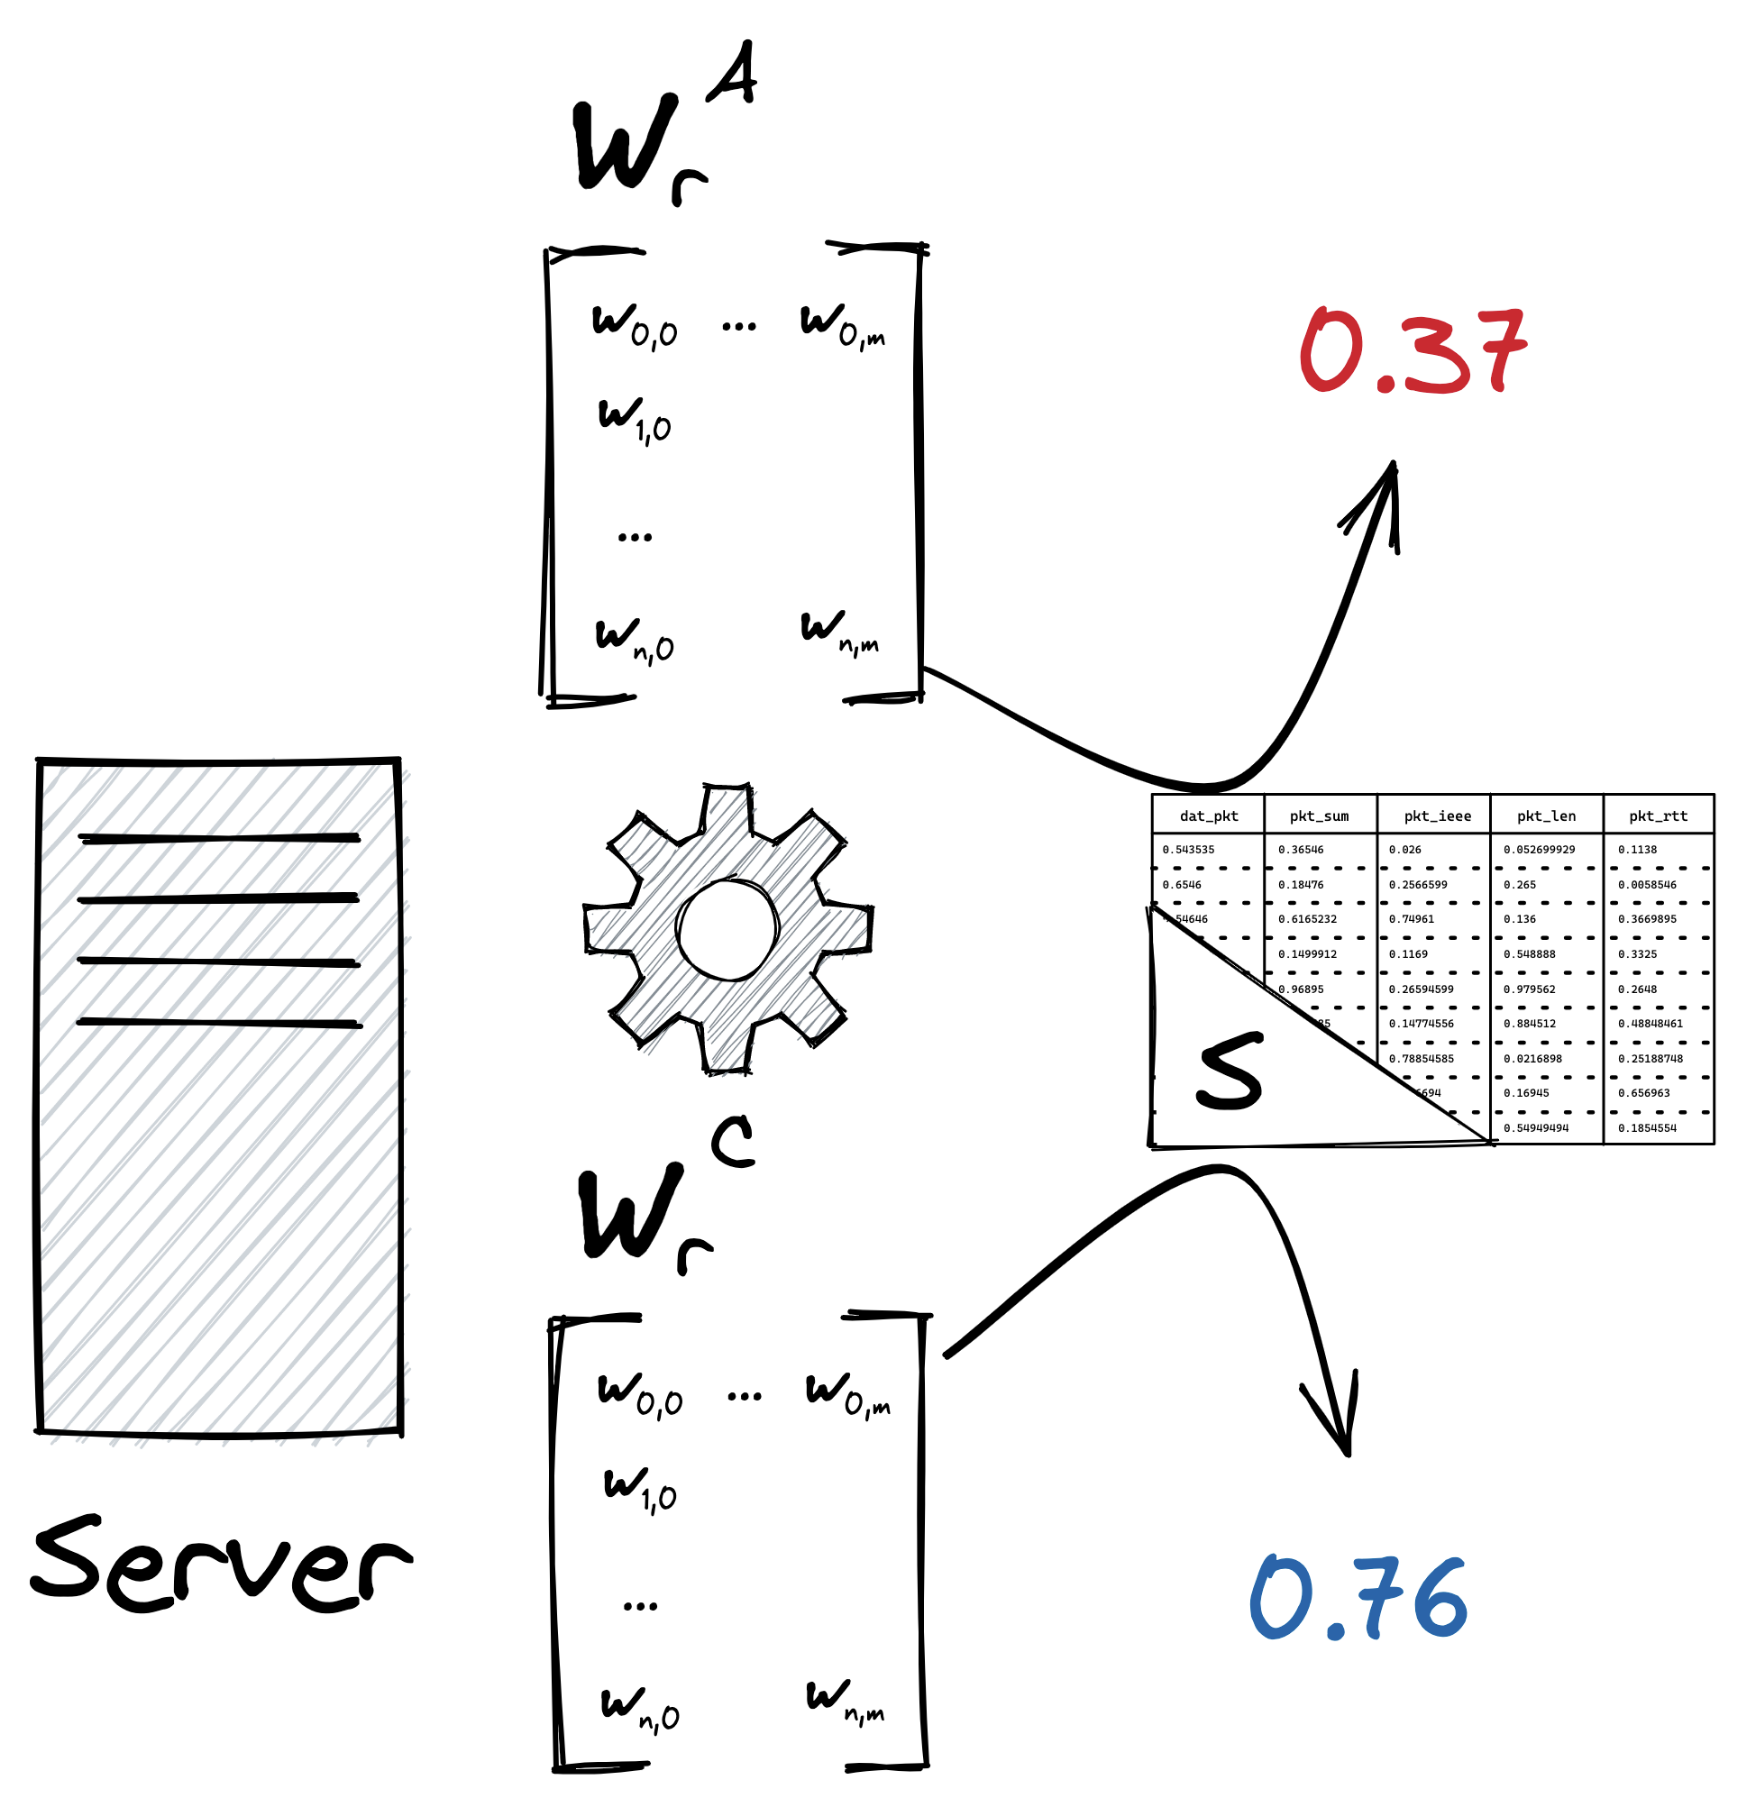
\includegraphics[height=.36\textheight]{figures/thesis/radar/server-side-eval}
%       \end{figure}

%       \begin{itemize}\footnotesize
%         \item Only applicable in IID settings.
%         \item Single source of truth.
%       \end{itemize}
%     \end{column}

%     \onslide<2->{%
%       \begin{column}{.33\textwidth}
%         \footnotesize\centering
%         \textbf{Server-side comparison}~\autocite{briggs_Federatedlearninghierarchical_2020}

%         \begin{figure}
%           \centering
%           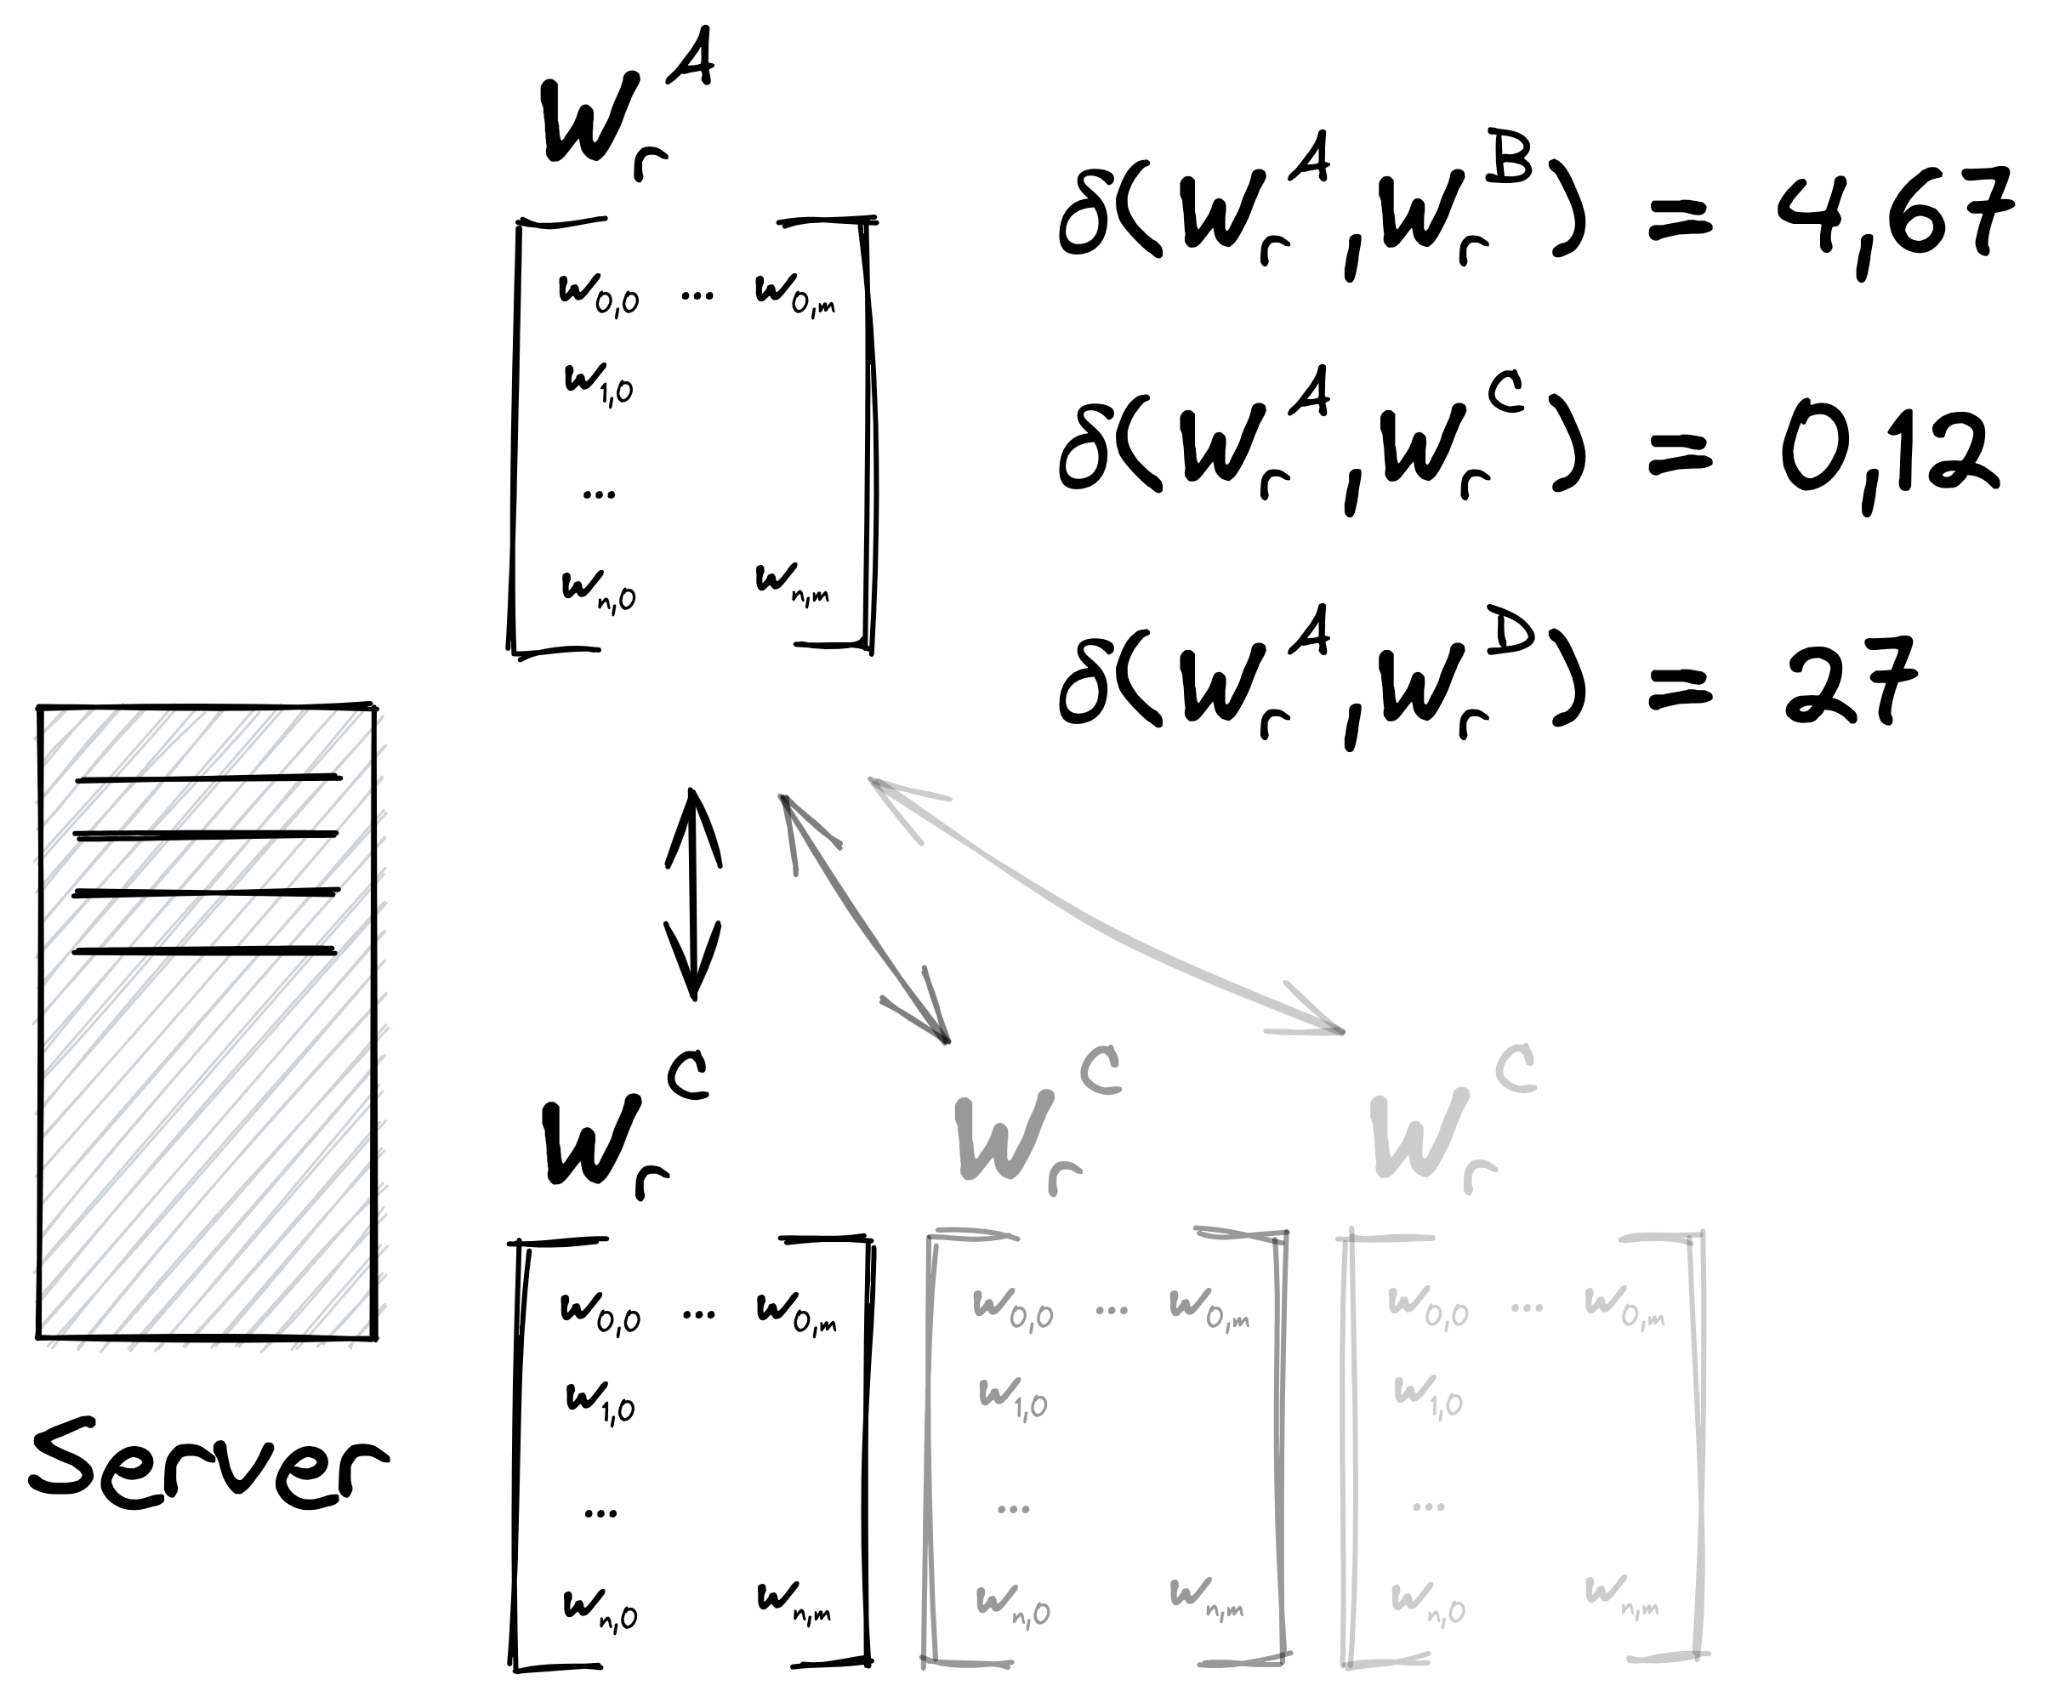
\includegraphics[height=.36\textheight]{figures/thesis/radar/server-side-comp}
%         \end{figure}

%         \begin{itemize}\footnotesize
%           \item Less related to client data.
%         \end{itemize}
%       \end{column}%
%     }

%     \onslide<3->{%
%       \begin{column}{.33\textwidth}
%         \footnotesize\centering
%         \textbf{Client-side evaluation}~\autocite{zhao_ShieldingCollaborativeLearning_2020}

%         \begin{figure}
%           \centering
%           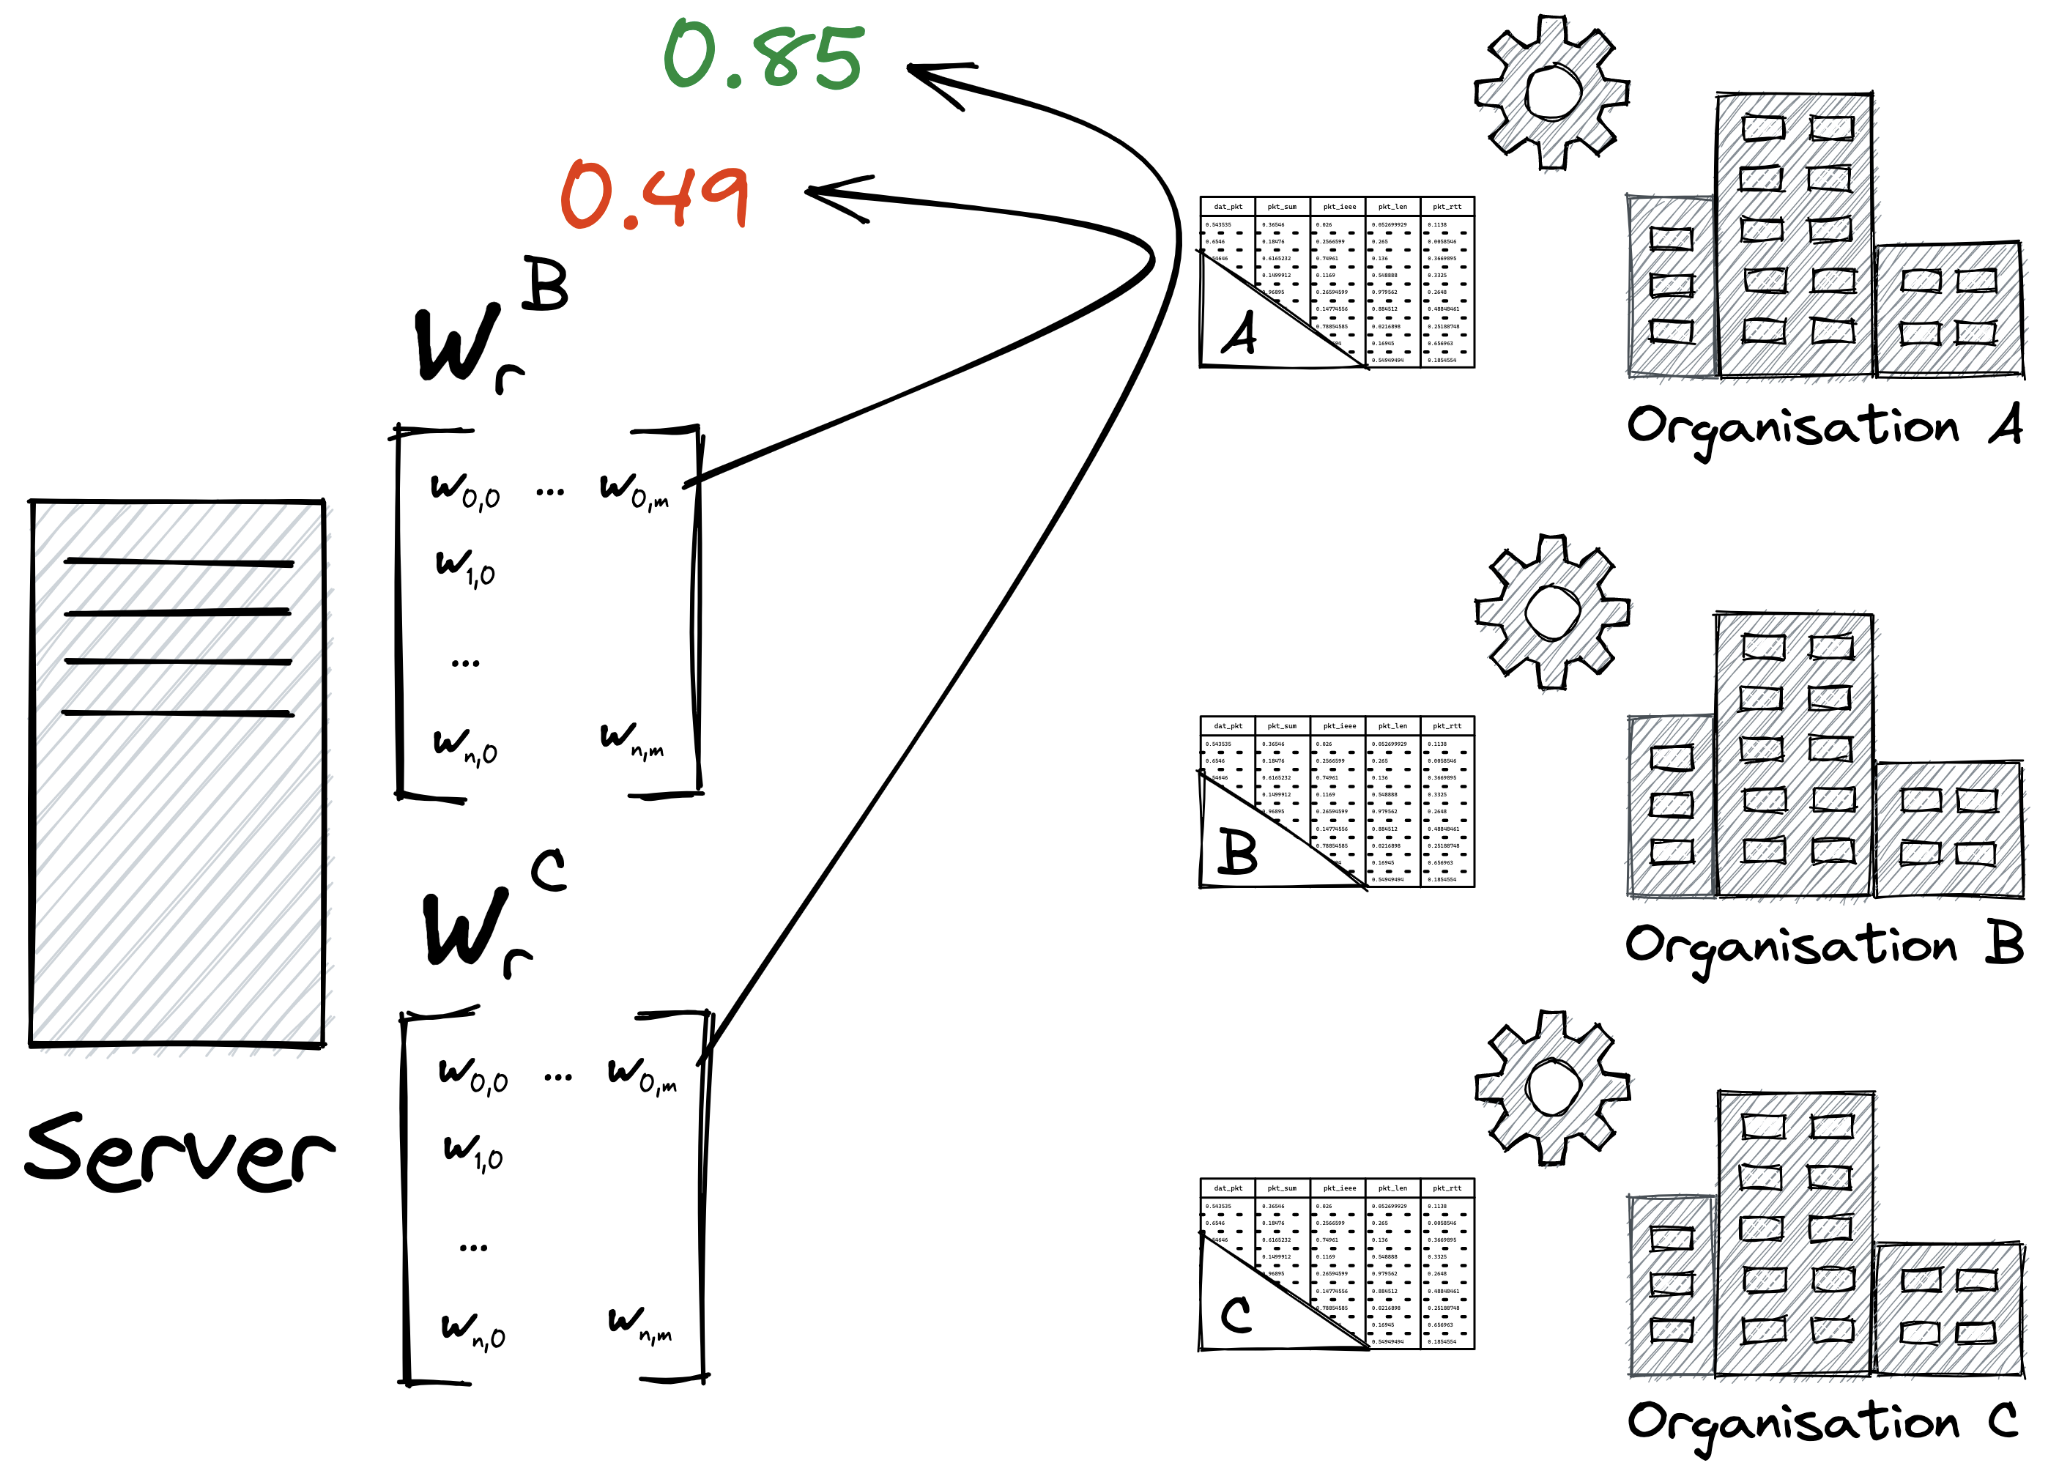
\includegraphics[height=.36\textheight]{figures/thesis/radar/client-side-eval}
%         \end{figure}

%         \begin{itemize}\footnotesize
%           \item High cost in cross-device.
%           \item More susceptible to badmouthing.
%         \end{itemize}
%       \end{column}%
%     }

%   \end{columns}

%   \vspace{3ex}
  
%   \footcite*{zhou_DifferentiallyPrivateFederated_2022}
%   \only<1>{\blankfootnote{}\blankfootnote{}\blankfootnote{}} % To keep the same height for the footnotes.
%   \only<2->{\footcite*{briggs_Federatedlearninghierarchical_2020}}
%   \only<2>{\blankfootnote{}}
%   \only<3->{\footcite*{zhao_ShieldingCollaborativeLearning_2020}}

% \end{frame}
% \endgroup

\begin{frame}{Introducing \texttt{RADAR}}
  \centering
    \begin{figure}
      \centering
      \foreach \i in {1,...,4} {
        \includegraphics<\i>[width=.95\linewidth,left]{figures/thesis/radar/agenda/\i.pdf}%
      }
      \vspace{-2em}
      \caption{\texttt{RADAR}~\footcite{lavaur_radar_2024} architecture, combining \emph{subjective} clustering and reputation-weighted aggregation to mitigate the impact lower-quality contributions.}
      \label{fig:radar}
    \end{figure}  
\end{frame}

% \begin{frame}{Assessing Quality with Cross-Evaluation}

%   \begin{columns}
%     \begin{column}{.45\textwidth}
%       \begin{figure}
%         \centering
%         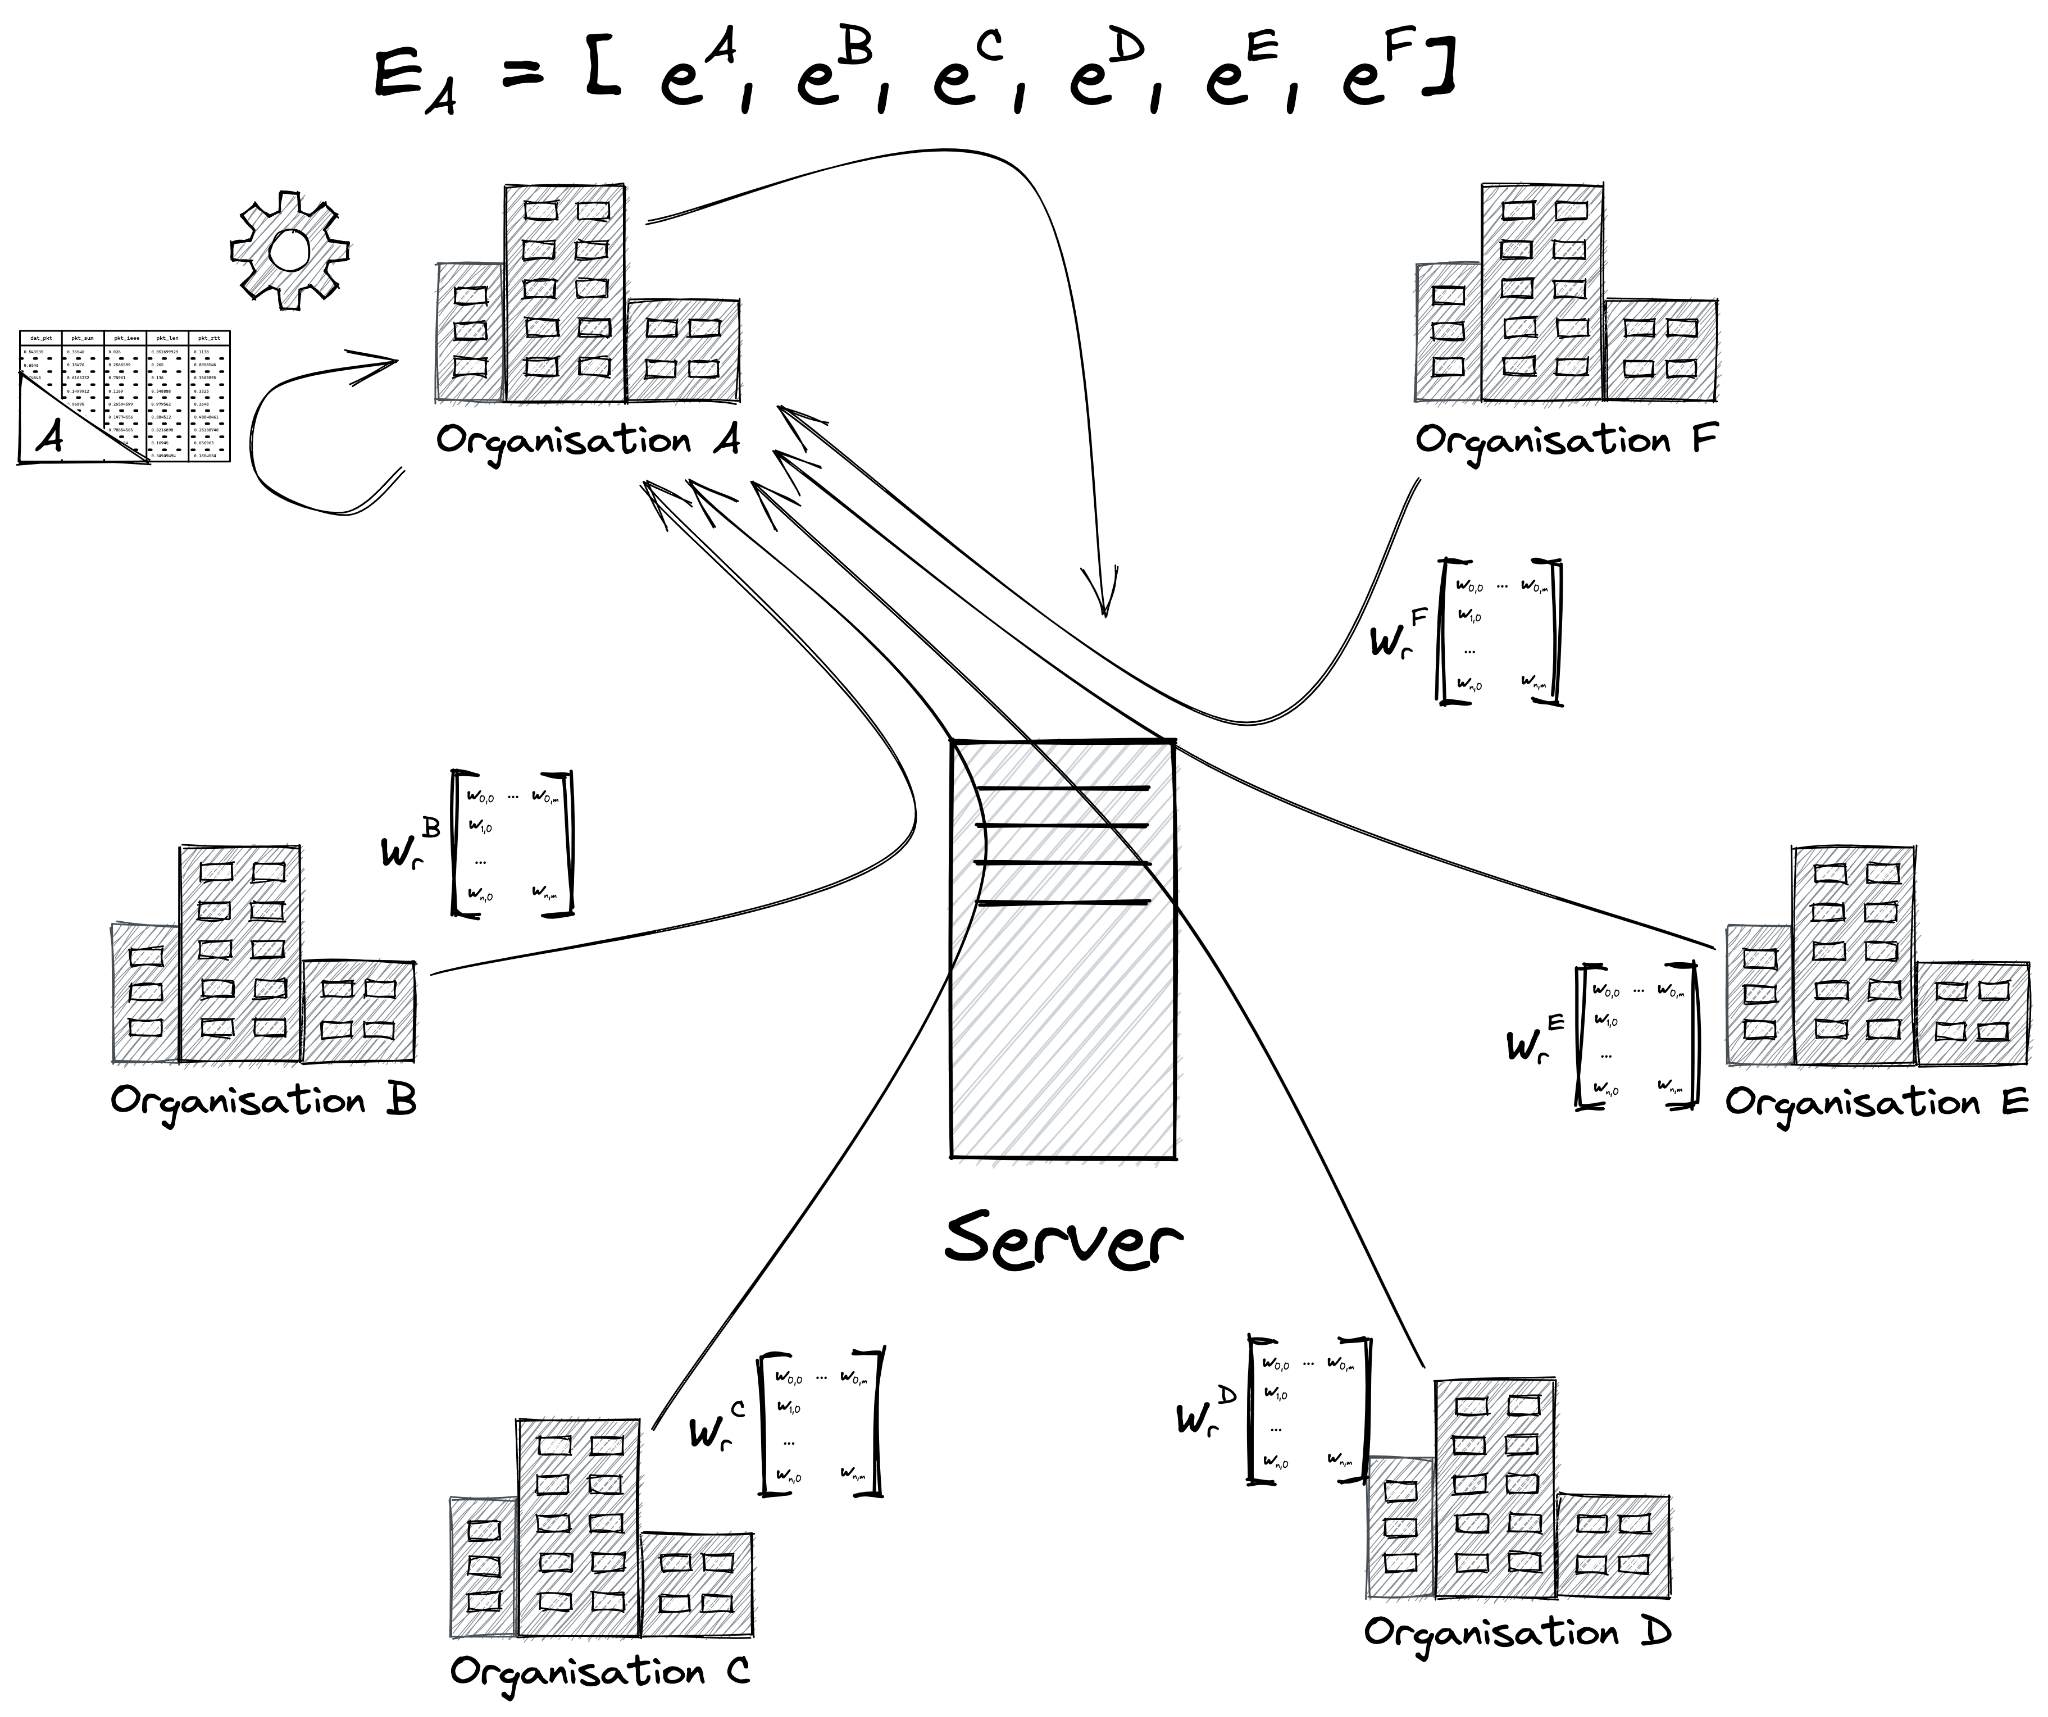
\includegraphics[width=\textwidth]{figures/thesis/radar/xeval}
%       \end{figure}
%     \end{column}
    
%     \begin{column}{.55\textwidth}
%       \footnotesize
%       \setlength{\baselineskip}{0.8\baselineskip}
%       \vspace{1ex}

%       \textbf{Advantages}
%       \begin{itemize}
%         \item Exhaustive overview of the entire system at each round $r$. \alert{No prior knowledge!}
%         \item Evaluations (\eg, accuracy, F1 score) representative of participants' data.
%       \end{itemize}
%       \medskip
%       \pause
%       \textbf{Drawbacks}
%       \begin{itemize}
%         \item High communication and computation costs.
%         \item Does not scale well.
%       \end{itemize}
%       \medskip
%       \pause
%       \textbf{But\dots}
%       \begin{itemize}
%         \item Cross-silo use case: few clients, with reasonable computing capacity.
%         \item Slow workflow: long time between rounds.
%       \end{itemize}
%     \end{column}

%   \end{columns}

% \end{frame}



% \begin{frame}{Fighting Heterogeneity with Clustering}
%   \bigskip\bigskip
%   \centering
%   \begin{minipage}{.8\textwidth}
%     \textbf{Objective}
%     \begin{itemize}
%       \item Build \emph{more} homogeneous communities of participants to facilitate model aggregation.
%     \end{itemize}    
%   \end{minipage}

  
%   \begin{columns}
%     \begin{column}{.5\textwidth}
%       \pause
%       \begin{itemize}
%         \item Distance metric
%         \begin{itemize}
%             \item Based on \alert{cross-evaluation} results. 
%             \item \alert{Cosine similarity}~\autocite{briggs_Federatedlearninghierarchical_2020}.
%         \end{itemize}
%       \end{itemize}
      
%       \pause
%       \begin{itemize}
%         \item Algorithm
%         \begin{itemize}
%           \item \alert{Hierarchical clustering}.~\autocite{briggs_Federatedlearninghierarchical_2020}
%           \item Dynamic aggregation threshold. 
%         \end{itemize}
%       \end{itemize}
%     \end{column}


%       \begin{column}{.5\textwidth}
%         \begin{figure}
%           \centering
%           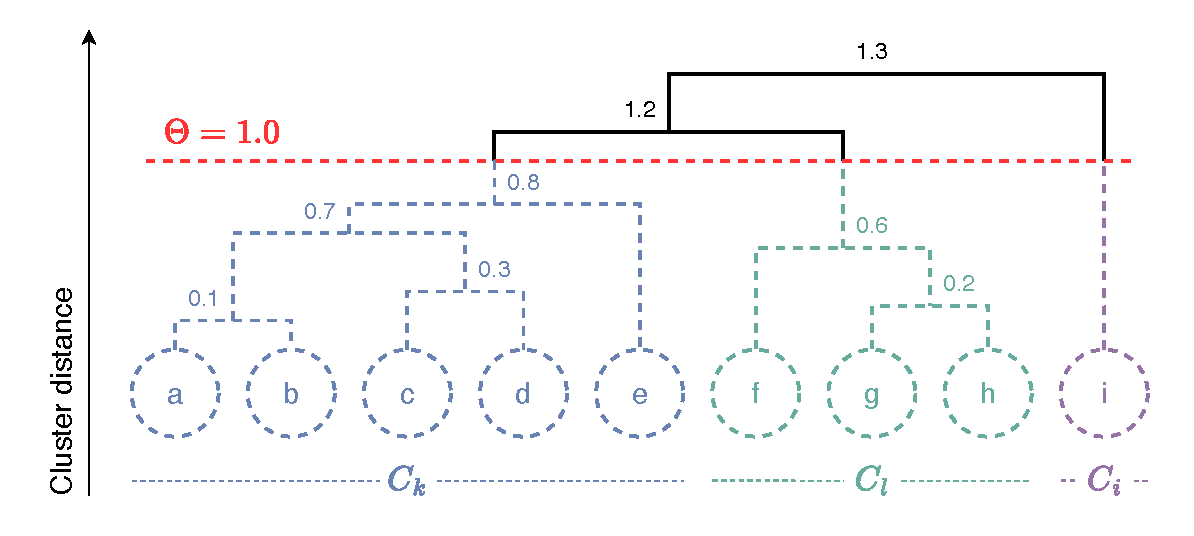
\includegraphics[width=\textwidth]{figures/thesis/radar/clustering.drawio.pdf}
%           \caption{Hierarchical clustering.}
%         \end{figure}
%       \end{column}
%   \end{columns}
%   \bigskip
%   \only<2->{\footcite*{briggs_Federatedlearninghierarchical_2020}}

% \end{frame}

% \begin{frame}{Reputation-aware Aggregation}
%   \begin{block}{Definition: Reputation Systems\normalfont~\autocite{resnick_Reputationsystems_2000}}
%     \begin{itemize}
%       \item Long-lived entities expecting future interaction.
%       \item Capture and distribution of feedback about current interactions (such information must be visible in the future).
%       \item Use of feedback to guide trust decisions.
%     \end{itemize}
%   \end{block}
%   \footcite*{resnick_Reputationsystems_2000}

%   % \pause
%   % \begin{itemize}
%   %   \item Votes weighted by the similarity inside each cluster.
%   %   \item Exponential decay for potential redemption.
%   % \end{itemize}

% \end{frame}

% \begin{frame}{Setup: Simulating Practical Heterogeneity}

%     \begin{columns}
%       \begin{column}{.4\textwidth}
%         \textbf{Datasets}
%         \begin{itemize}
%           \item Heterogeneous datasets, but some participants can share similarities.
%           \item 4 datasets: CIC-CSE-IDS2018, UNSW-NB15, Bot-IoT, ToN\_IoT.
%           \item NF-V2~\autocite{sarhan_StandardFeatureSet_2021} feature set (\ie, NetFlow V9).
%         \end{itemize}
%       \end{column}
%       \begin{column}{.56\textwidth}
%         \begin{figure}
%           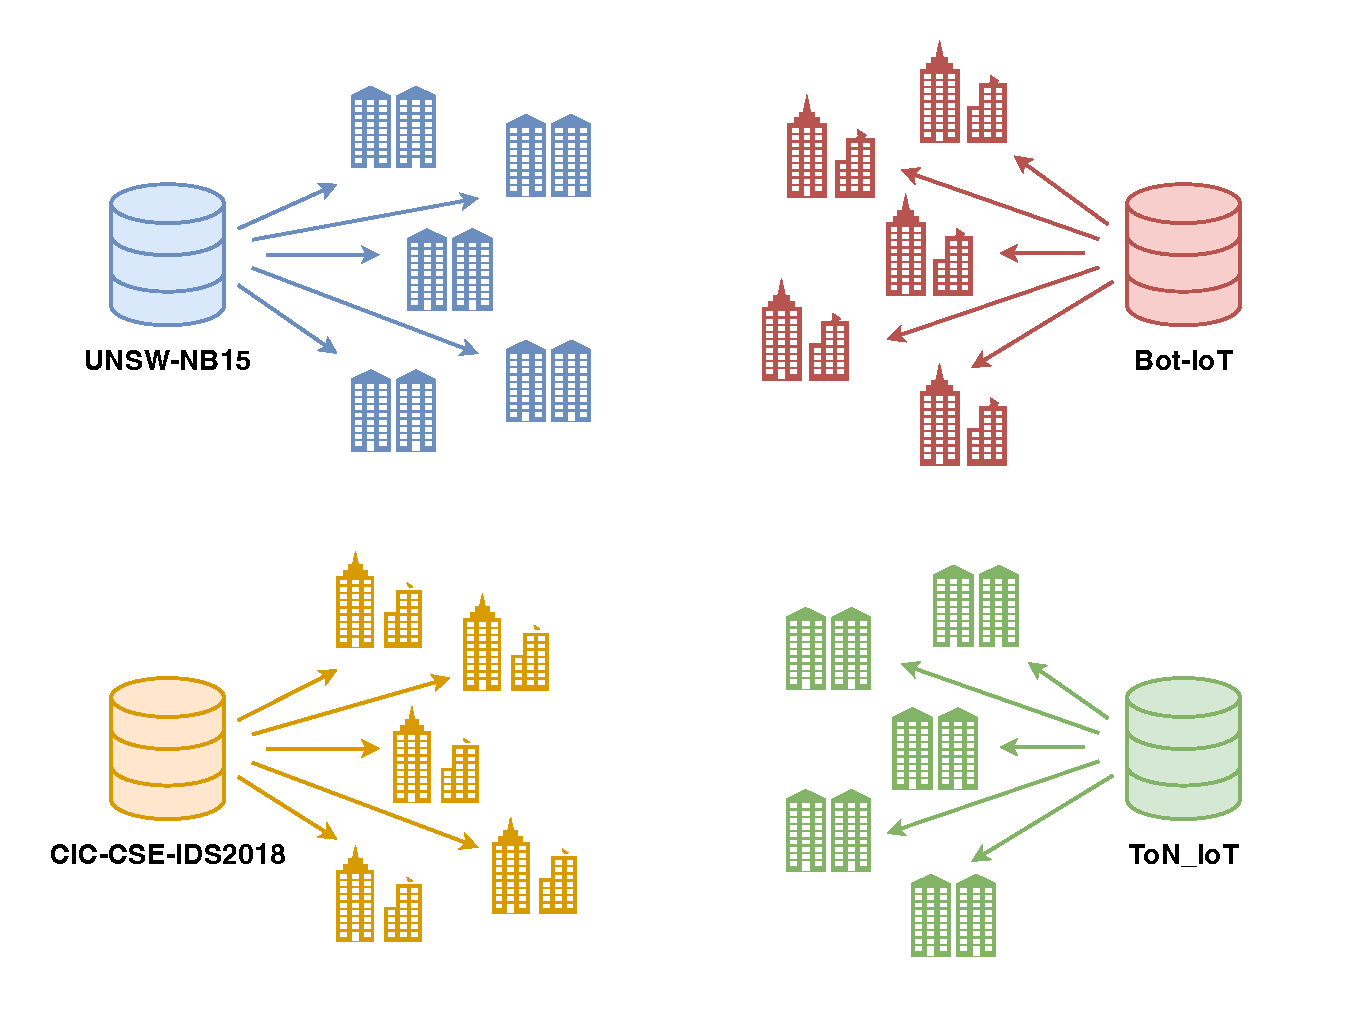
\includegraphics[width=\linewidth]{figures/thesis/radar/partition.pdf}%
%         \end{figure}
%       \end{column}
%     \end{columns}
%     \footcite*{sarhan_StandardFeatureSet_2021}
%   \end{frame}
  
  % \begin{frame}{Setup: Byzantine Scenarios}
  %     \begin{columns}
  %         \begin{column}{.4\textwidth}
  %             \textbf{Parameters}
  %             \begin{itemize}
  %                 \item \textit{Target}: Affected classes.
  %                 \item \textit{Data Poisoning Rate (DPR)}: proportion of targeted data with flipped labels.
  %                 \item \textit{Model Poisoning Rate (MPR)}: number of attackers in the cluster.
  %             \end{itemize}
  %         \end{column}
  %         \begin{column}{.56\textwidth}
  %           \begin{figure}
  %             \captionsetup{font=small, labelfont=small}
  %             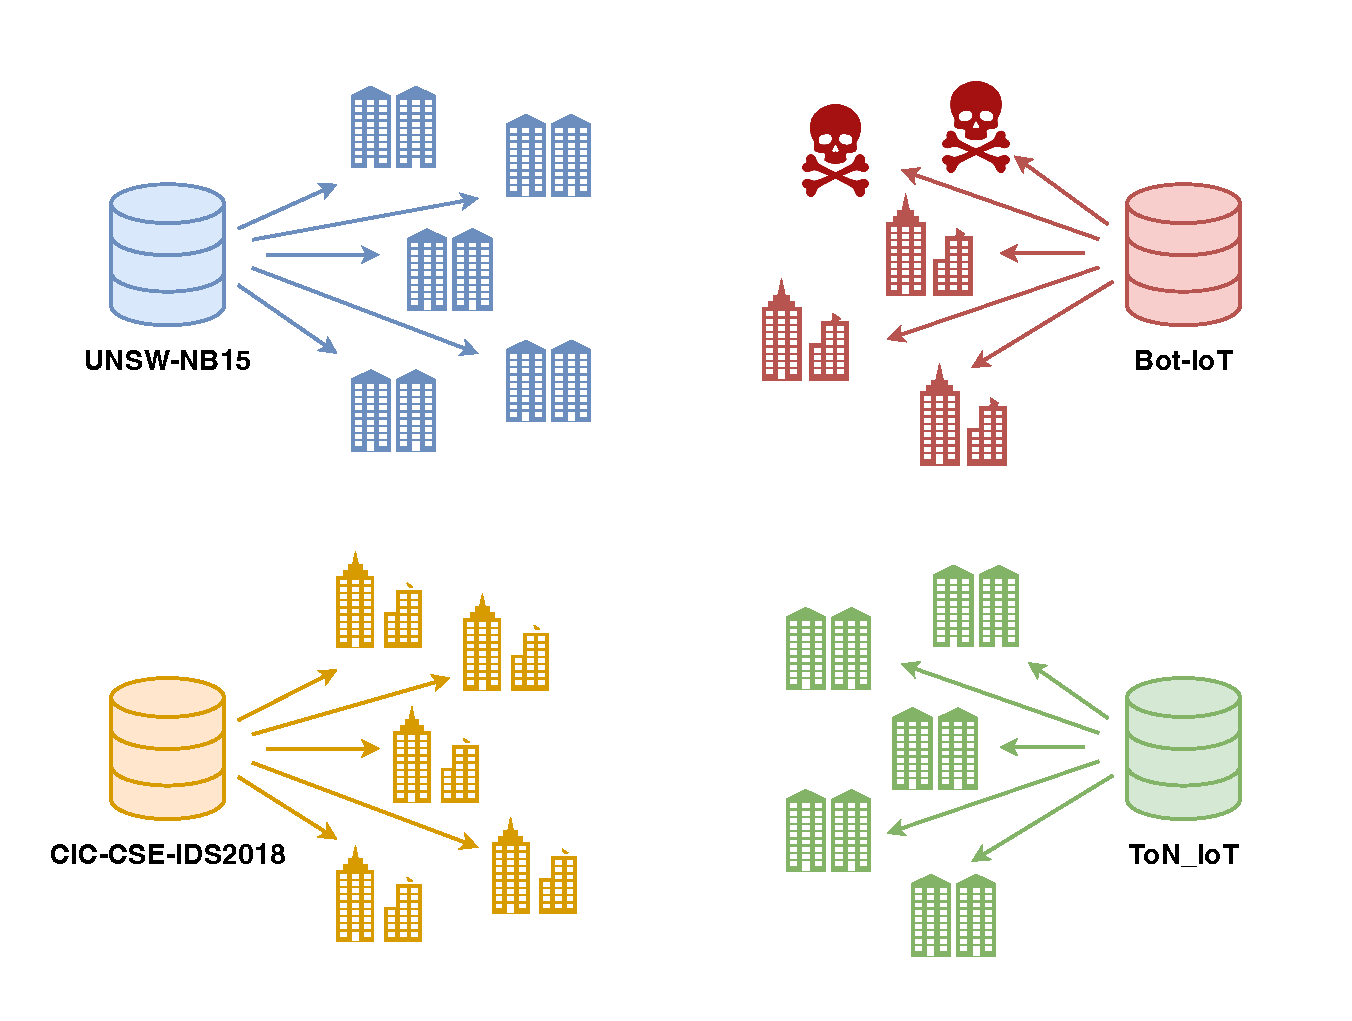
\includegraphics[width=\linewidth]{figures/thesis/radar/poisoning.pdf}%
  %             \captionsetup{justification=centering}
  %             \caption*{
  %               \texttt{colluding minority 100T}\\
  %               \footnotesize (\ie, 2 attackers, 100\% DPR on Reconnaissance class).
  %             }
  %           \end{figure}
  %         \end{column}
  %     \end{columns}
  % \end{frame}

% \begin{frame}{Results}
%   \begin{columns}
%     \column{.5\textwidth}
%     \begin{figure}
%       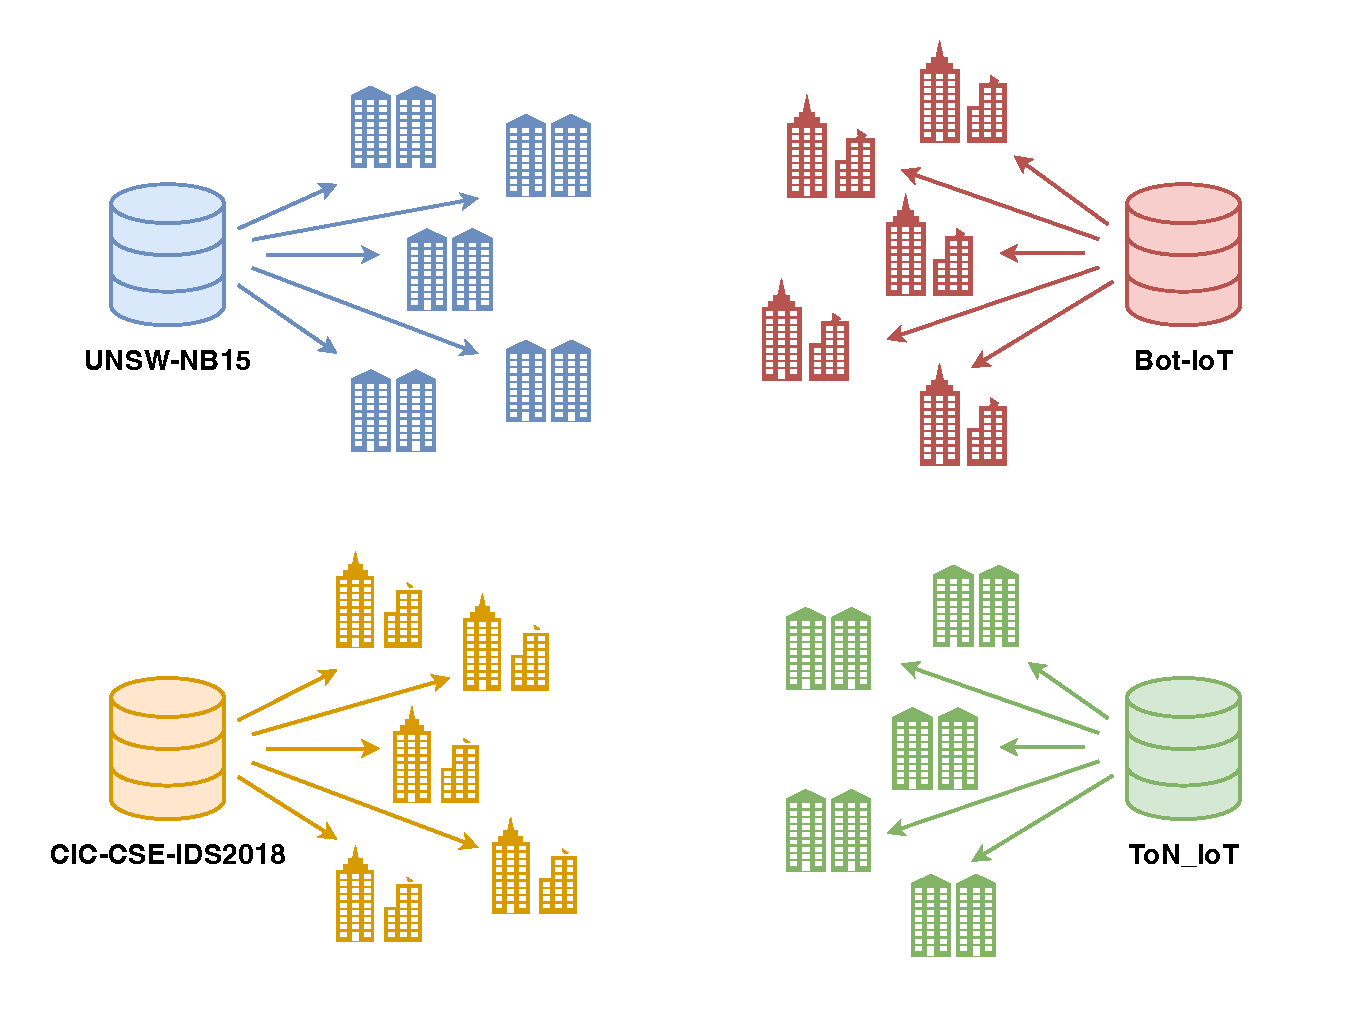
\includegraphics[width=.9\linewidth]{figures/thesis/radar/partition.pdf}%
%       \caption{Emulating heterogeneity using unified feature set on multiple datasets.}
%     \end{figure}

%     \column{.5\textwidth}
%     \renewcommand{\hl}{\cellcolor{white}}
%     \only<2>{\renewcommand{\hl}{\cellcolor{green!30}}}
%     \begin{table}
%       \centering
%       \caption{
%         \textit{Effect of different attack configurations (untargeted) on all baselines.}
%         \texttt{RA} is RADAR, \texttt{FG} is \texttt{FoolsGold}, \texttt{FA} is \texttt{FedAvg} (on \textit{all} participants), and \texttt{FC} is \texttt{FedAvg} ideally clustered per dataset.
%       }
%       \footnotesize
%       \setlength\tabcolsep{1ex}
%       \begin{tabularx}{\textwidth}{l>{\raggedright\arraybackslash}p{2.15cm}|rrrr}
%         \toprule % ---------------------------------
%         \multicolumn{2}{c|}{\multirow{2}{*}{\textbf{Scenario}}} & \multicolumn{4}{c}{\textbf{\gls{asr}} (\%, \textit{lower is better})} \\
%         & & \multicolumn{1}{c}{\texttt{RA}} & \multicolumn{1}{c}{\texttt{FG}} & \multicolumn{1}{c}{\texttt{FA}} & \multicolumn{1}{c}{\texttt{FC}} \\
%         \midrule % ---------------------------------
%         % TARGETED ATTACKS
%         \multicolumn{2}{l|}{\textbf{Targeted} (\texttt{100T})} & & & & \\
%           & \hl \texttt{Benign}       &  \hl \textbf{0.00} &  5.17 & 5.10 &  0.09 \\
%           & \hl \texttt{Lone}         &  \hl \textbf{0.00} & 93.82 & 6.73 &  0.45 \\
%           & \hl \texttt{Collud.~min.} &  \hl \textbf{0.00} &  2.97 & 9.99 & 53.40 \\
%           & \only<3>{\cellcolor{red!20}} \texttt{Collud.~maj.} &  \only<3>{\cellcolor{red!20}} 73.39 & \textbf{8.10} & 17.65 & 59.36 \\
%         \midrule % ---------------------------------
%         % UNTARGETED ATTACKS
%         \multicolumn{2}{l|}{\textbf{Untargeted} (\texttt{100U})} & & & & \\
%         & \hl \texttt{Benign}        & \hl 0.09  & 0.39 & 33.30 & \textbf{0.06} \\
%         & \hl \texttt{Lone}          & \hl \textbf{0.08} & 99.89 & 54.70 & 0.12 \\
%         & \hl \texttt{Collud.~min.}  & \hl 0.10 & \textbf{0.04} & 44.53 & 6.26 \\
%         & \hl \texttt{Collud.~maj.}  & \hl \textbf{0.08} & 38.98 & 59.49 & 94.36 \\
%         \bottomrule% ---------------------------------
%       \end{tabularx}
%     \end{table}
%   \end{columns}
% \end{frame}

\newcommand{\hr}{\cellcolor{red!30}}
\newcommand{\ho}{\cellcolor{orange!30}}
\newcommand{\hg}{\cellcolor{green!30}} 

\begin{frame}{Handling heterogeneity}
  \begin{columns}
    \begin{column}{.4\textwidth}
      \begin{figure}
              \captionsetup{justification=centering}
        \includegraphics<1>[width=\linewidth,left]{./figures/radar-eval/clustering/clustering_benign.pdf}%
        \caption{Clustering results without poisoning.\\ 
        Rand index=1.0}
      \end{figure}
    \end{column}
  \begin{column}{.6\textwidth}

\begin{table}
    \centering
    \caption*{Accuracy for different baselines.}
    \footnotesize
    \setlength\tabcolsep{1ex}
    \begin{tabularx}{.7\textwidth}{>{\raggedright\arraybackslash}p{2.15cm}|ccc}
      \toprule % ---------------------------------
      \textbf{Scenario}
      & \multicolumn{1}{c}{\texttt{RADAR}} & \multicolumn{1}{c}{\texttt{FoolsGold}} & \multicolumn{1}{c}{\texttt{Clustered}} \\
      \midrule % ---------------------------------
      \textbf{Benign} & \hg 99.07 & \hr 55.04 & \hg 99.24  \\
    \end{tabularx}
    \caption*{\footnotesize More is better}

  \end{table}
    \end{column}
  \end{columns}
\end{frame}

%%%%%%%%%%%%
%Untargeted
%%%%%%%%%%%%
\begin{frame}{Handling Untargeted Byzantines}
  \begin{columns}
    \begin{column}{.4\textwidth}
      \begin{figure}
        \captionsetup{justification=centering}
        \only<1>{
            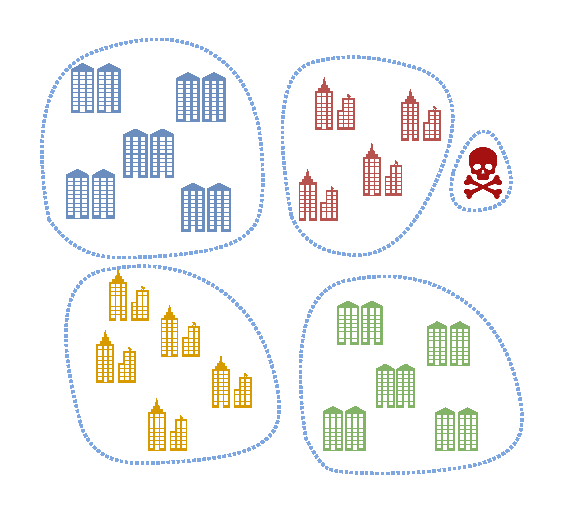
\includegraphics[width=\linewidth,left]{./figures/radar-eval/clustering/clustering_lone_untargeted.pdf}
            \caption*{Clustering results for\\
            \texttt{lone 100U}.\\ 
            Rand index=1.0
            }
        }
        \only<2>{
            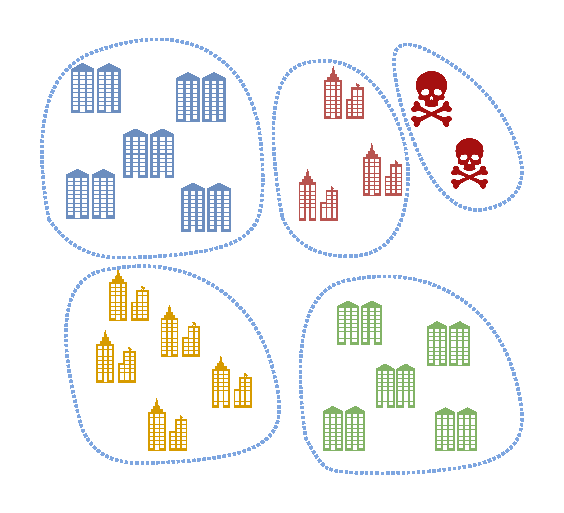
\includegraphics[width=\linewidth,left]{./figures/radar-eval/clustering/clustering_min_untargeted.pdf}
            \caption*{Clustering results for\\ \texttt{colluding minority 100U}\\ 
            Rand index=1.0
            }
        }
        \only<3>{
            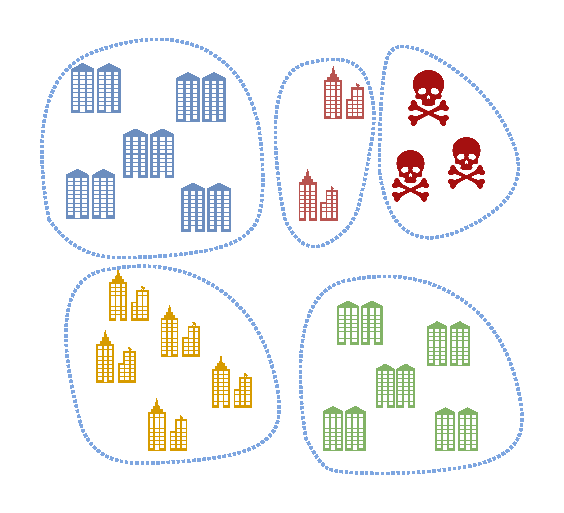
\includegraphics[width=\linewidth,left]{./figures/radar-eval/clustering/clustering_maj_untargeted.pdf}
          \caption*{Clustering results for\\
            \texttt{colluding majority 100U}\\ 
            Rand index=1.0
            }
        }        
      \end{figure}
    \end{column}

  \begin{column}{.6\textwidth}
    \begin{table}
        \centering
    
        \footnotesize
        \setlength\tabcolsep{1ex}
        \caption*{Attack success rate for different baselines.}  
        \begin{tabularx}{.8\textwidth}{l>{\raggedright\arraybackslash}p{2.15cm}ccc}
          \toprule % ---------------------------------
          \multicolumn{2}{c}{{\textbf{Scenario}}}
          & \multicolumn{1}{c}{\texttt{RADAR}} & \multicolumn{1}{c}{\texttt{FoolsGold}} & \multicolumn{1}{c}{\texttt{Clustered}} \\
          \midrule % ---------------------------------
          % % UNTARGETED ATTACKS
          \multicolumn{2}{l}{\textbf{Untargeted} (\texttt{100U})}  & & & \\
          & \texttt{Lone} & \hg 0.08 &\hr 99.89 & \hg 0.12 \\
          \only<2->{& \texttt{Collud. min.} & \hg 0.10 & \hg 0.04 &\ho 6.26 \\}
          \only<3->{& \texttt{Collud. maj.} & \hg 0.08 &\ho 38.98 & \hr 94.36 \\}
          \end{tabularx}
          \caption*{\footnotesize Less is better}
      \end{table}
  
     \end{column}
  \end{columns}
\end{frame}


%%%%%%%%%%%%    
% Targeted   
%%%%%%%%%%%%

\begin{frame}{Handling Targeted Byzantines}
    \begin{columns}
        \begin{column}{.4\textwidth}
            \begin{figure}
                \centering
                \captionsetup{justification=centering}
                \only<1-2>{%
                    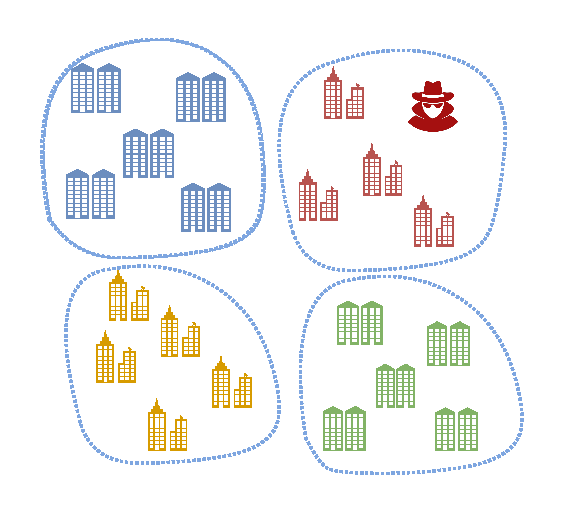
\includegraphics[width=\linewidth,left]{figures/radar-eval/clustering/clustering_lone_targeted.pdf}
                    \caption*{
                        Clustering results for\\
                        \texttt{Lone 100T}\\ 
                        Rand index=0.97
                    }
                }
                \only<3>{%
                    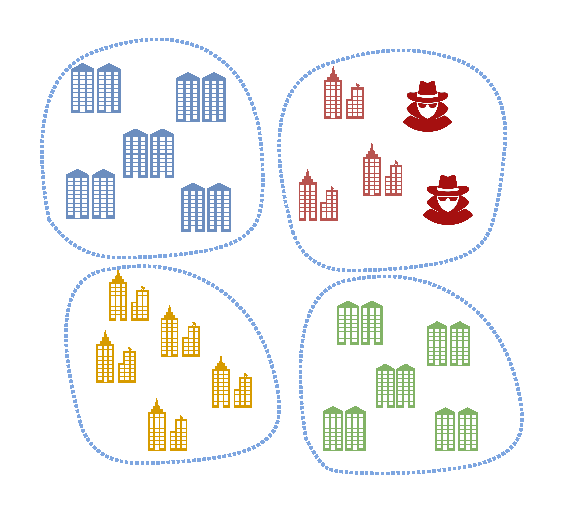
\includegraphics[width=\linewidth,left]{./figures/radar-eval/clustering/clustering_min_targeted.pdf}%
                    \caption*{
                        Clustering results for\\
                        \texttt{colluding minority 100T}\\ 
                        Rand index=0.97
                    }
                }
                \only<4>{
                    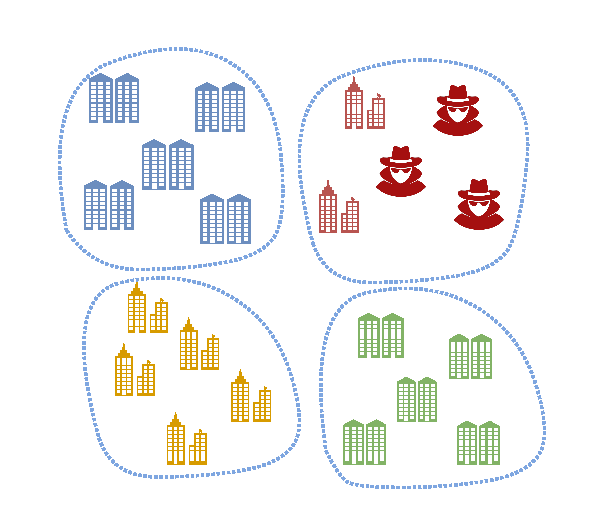
\includegraphics[width=\linewidth,left]{./figures/radar-eval/clustering/clustering_maj_targeted.pdf}%
                    \caption*{Clustering results for \texttt{colluding majority 100T}\\ 
                    Rand index=0.96}
                }
                
            \end{figure}
        \end{column}
        \begin{column}{.6\textwidth}
            \begin{table}
                \centering
                \footnotesize
                \setlength\tabcolsep{1ex}
                \caption*{Attack success rate for different baselines.}  

                \begin{tabularx}{.8\textwidth}{l>{\raggedright\arraybackslash}p{2.15cm}ccc}
                    \toprule % ---------------------------------
                    \multicolumn{2}{c}{{\textbf{Scenario}}}
                    & \multicolumn{1}{c}{\texttt{RADAR}} & \multicolumn{1}{c}{\texttt{FoolsGold}} & \multicolumn{1}{c}{\texttt{Clustered}} \\
                    \midrule % ---------------------------------
                    % % TARGETED ATTACKS
                    \multicolumn{2}{l}{\textbf{Targeted} (\texttt{100T})}  & & & \\    
                    & \texttt{Lone} &\hg 0.00 & \hr 93.82 & \hg 0.45 \\
                    \only<3->{& \texttt{Collud. min.} & \hg 0.00 & \hg 2.97 & \hr 53.40 \\}
                    \only<4->{& \texttt{Collud. maj.} &  \hr 73.39 & \ho 8.10 & \hr 59.36 \\}
                \end{tabularx}
                
                \caption*{\footnotesize Less is better}
            \end{table}
            \vspace{-1em}
            
            \only<2>{\begin{minipage}{\textwidth}
                \begin{figure}
                    \captionsetup{justification=centering}
                    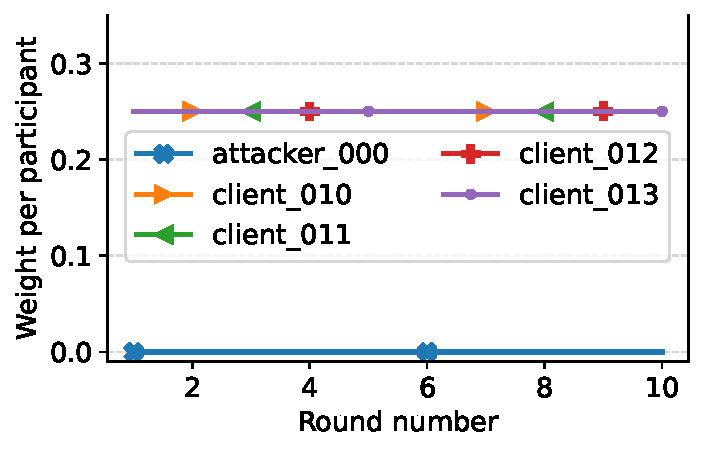
\includegraphics[width=.6\linewidth]{./figures/radar-eval/reput/lone_loud_expanded.pdf}
                    \caption{Aggregation weights.}
                \end{figure}
            \end{minipage}}

          %   \only<5>{\begin{minipage}{\textwidth}
          %       \begin{figure}
          %           \captionsetup{justification=centering}
          %           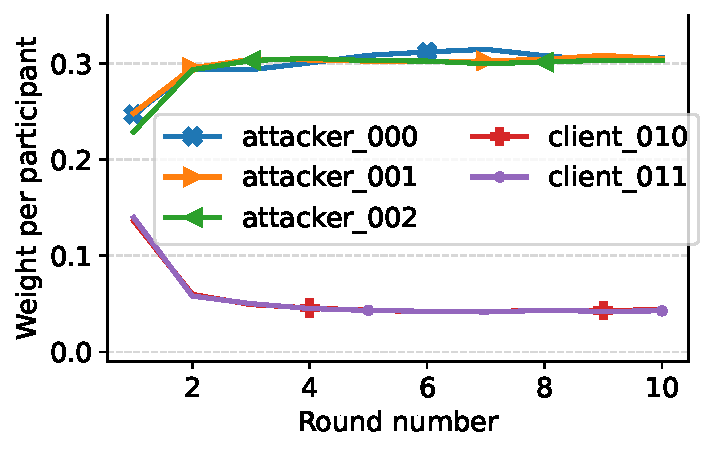
\includegraphics[width=.6\linewidth]{./figures/radar-eval/reput/byzantine_majority_loud_expanded.pdf}
          %           \caption{Aggregation weights.}
          %       \end{figure}
          %  \end{minipage}}

        \end{column}
    \end{columns}
\end{frame}



\begin{frame}{Highlights}
  % \begin{block}{Combining clustering and mitigation strategy is effective}
  %   Clustering effectively creates \alert{homogeneous} communities where conventional mitigation can be applied.
  % \end{block}

  % \pause
  \begin{block}{Cross-evaluation enable \alert{true} reputation-aware FL}
    Only way to gather indirect feedbacks (\ie, one clients' evaluation of another's contribution); at the cost of scalability.
  \end{block}

  \pause
  \begin{block}{Generalizable outside intrusion detection}
    With a few conditions: parametric models, locally owned evaluation set, a \alert{small-scale use case}, and a \alert{trusted central server}.
  \end{block}
\end{frame}

% \begin{frame}{Takeways}
%   \begin{enumerate}
%     \onslide<+->
%     \item \texttt{RADAR} can:
%     \begin{itemize}
%       \item leverage \alert{cross-evaluation}, \alert{clustering} and \alert{reputation} to address heterogeneity and Byzantine contributions;
%       \item adjust rapidly to changes in behavior; and
%       \item mitigate most tested scenarios (limiting case handled up to 80\% of poisoned data).
%     \end{itemize}

%     \medskip
%     \onslide<+->
%     \item How generic?
%     \begin{itemize}
%       \item Only few conditions: parametric models, locally owned evaluation set, a \alert<+->{small-scale use case}, and a \alert<.->{trusted central server}.
%     \end{itemize}

%     \medskip
%     \onslide<+->
%     \item Future works:
%     \begin{itemize}
%       \item Remove the central server dependency for \alert{increased trust and scalability}.
%       \item Test the approach in more realistic heterogeneous settings.
%     \end{itemize}
%   \end{enumerate}

% \end{frame}